% EPC flow charts
% Author: Fabian Schuh
\documentclass{article}
\usepackage{myflowchart}

\begin{document}

\begin{tikzpicture}

\begin{scope}[node distance=5mm and 5mm]

\node [ item=2](a) at (1,1) {%
            \textbf{weekly routine}
            \nodepart{two}
            \begin{enumerate}
            	\item 最近在弄水平平台
	    \end{enumerate}
            };

\node [ item=2, below = of a](sustain) {%
            \textbf{self sustain}
            \nodepart{two}
            \begin{enumerate}
            	\item 由於體積開始變大,這代表這些東西的表面積開始指數增加,因此表面的work非常多,如何處理?
		\item 表面做了東西以後,若是新東西還要記錄(目前這一點做的不錯),若是發現過去方法有誤還要去修正過去的說明書(目前這一點進展很慢很慢,因為需要跟群組聯繫上,因此比較不容易)。
		\item if wanna venture more, better self sus, assess cll conditions again.
			\begin{enumerate}
				\item cargo container: call, search, ask $\circ\circ\circ$
				\item salun: bogged down due to container? $\bullet\circ\circ$
			\end{enumerate}
            \end{enumerate}
            };



\node [above right = of a, align = center, anchor = south] (title){\parbox[c][][c]{0.1\textwidth}{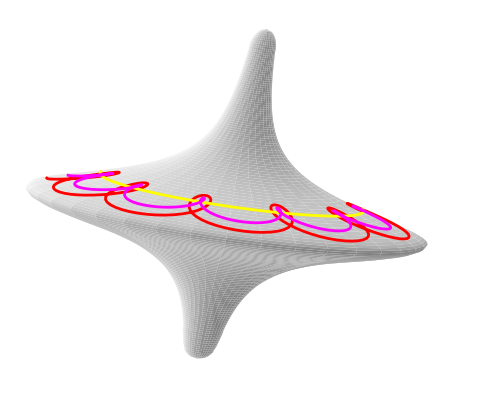
\includegraphics[width=0.1\textwidth]{../../figs/logo_June27_2016.png}}\parbox[c][][c]{7cm}{\Huge fixing \& crafting}};


\node [ item=2, below right = of title, anchor = north](small) {%
            \textbf{待完成}
            \nodepart{two}
            \begin{enumerate}
            	\item thinkpad T60 電池找
            	\item SMEG烤箱時間溫度表製作
            	\item compressor 排水閥, still no clue, dangerous
		\item 打氣筒要修,或許換打氣頭?
		\item 補褲$\bullet\bullet\bullet\circ$
		\item 相機,手機插電
		\item 電繡片問正興老闆
		\item note裝訂強力邊改良
		\item 印表機淡,修,感光鼓,電棒?
		\item 相機接ps
		\item 電動起子接ps
           \end{enumerate}
            };

\node [ item=2, below = of small](impossible) {%
            \textbf{大概無法完成了}
            \nodepart{two}
            \begin{enumerate}
            	\item 可繼續印以及可以擦掉的printer
		\item 調墨水,加墨水
            \end{enumerate}
            };

\node [ wideitem=2, below right = of sustain, anchor=north](machining) {%
            \textbf{金屬加工}
            \nodepart[text width = 16.5cm]{two}
            \begin{itemize}
            	\item 陀螺儀轉動框加工
		\item 車洗水平上下移動平台
		\begin{itemize}
            		\item 車洗要固定在桌上
			\item 桌子直角加強,需要切撿回來的木頭。但是上次試過不好切,因為一來切割圓盤不夠大,剖面方向無法整個切斷,得要縱向切一刀,再橫向切。這就需要可以固定住木頭的大型夾具,需要製作大型夾具。目前圓鉅機平台完成一半,尚未完成。
			\item 圓鉅機平台->切木頭->固定桌子->固定車洗->製作上下水平移動平台->加工轉動框。
			\item part holders大的小的,用甚麼做?
		\end{itemize}
            \end{itemize}
            };
\end{scope}
\end{tikzpicture}
\end{document}
